
\documentclass[preprint,12pt]{elsarticle}

\usepackage[spanish]{babel}
\usepackage{amssymb}
\usepackage{graphicx}
\usepackage{lineno}
\usepackage[utf8]{inputenc}
\usepackage{url}
\usepackage{natbib} 
\usepackage{amsmath} 
\usepackage{amssymb} 

\begin{document}
	
	\begin{frontmatter} 

		\title{\huge MAQUINAS VIRTUALES VS CONTENEDORES}
		
		\author{Huichi Contreras, Franklin Carlos            (2016056193)}
		\author{Gonzales Cave, Angel Gabriel                 (2017057861)}
		\author{Condori Quispe, Yhónn Joel	         	   (2016056358)} 
		\author{Pastor Mendoza, José Edilberto              (2016055237)} 
		\address{Escuela Profesional de Ingeniería de Sistemas}
		\address{Universidad Privada de Tacna}
		\address{Tacna, Perú}
		
%% ABSTRACT --------------------------------------------------------------------------------------------------------------------

		\begin{abstract}
Lorem Ipsus

		\end{abstract}

%% ----------------------------------------------------------------------------------------------------------------------------------

	\end{frontmatter}

%% RESUMEN ---------------------------------------------------------------------------------------------------------------------

\section{Resumen}
Lorem Ipsus


%% ----------------------------------------------------------------------------------------------------------------------------------


%% INTRODUCION ----------------------------------------------------------------------------------------------------------------

\section{Introducción} 

Lorem Ipsus

%% ----------------------------------------------------------------------------------------------------------------------------------


%% TITULO  ------------------------------------------------------------------------------------------------------------

\section{Título}

Lorem Ipsus
%% ----------------------------------------------------------------------------------------------------------------------------------

%% AUTORES  ------------------------------------------------------------------------------------------------------------

\section{Autores}

\begin{table}[htbp]
\begin{center}
\begin{tabular}{|l|l|}
\hline
Roles & Integrantes \\
\hline \hline
Product owner & Gonzales Cave, Angel Gabriel \\ \hline
Scrum master & Huichi Contreras, Franklin Carlos  \\ \hline
Equipo scrum & Condori Quispe, Yhónn Joel | Pastor Mendoza, José Edilberto \\ \hline
\end{tabular}
\caption{Integrantes del equipo}
\label{tabla:sencilla}
\end{center}
\end{table}


%% ----------------------------------------------------------------------------------------------------------------------------------

%% PLANTEAMIENTO DEL PROBLEMA ------------------------------------------------------------------------------------------------------------

\section{Planteamiento del problema}
Lorem Ipsus

%%  SUBSECCION 

\subsection {\textbf{Problema}}
Lorem Ipsus

%%  SUBSECCION 

\subsection {\textbf{Justificacion}}

Lorem Ipsus

%%  SUBSECCION 

\subsection {\textbf{Alcance}}
Lorem Ipsus

%% ----------------------------------------------------------------------------------------------------------------------------------

%% OBJETIVOS ------------------------------------------------------------------------------------------------------------

%%  SUBSECCION 

\subsection{\textbf{General}}

Lorem Ipsus

%%  SUBSECCION 

\subsection{\textbf{Especificos}}

\begin{itemize}

\item Analizar cuáles son las peticiones de soporte técnico mas solicitadas por los usuarios, para obtener la informacion necesaria y definir los requerimientos para el correcto desarrollo del sistema
\item Mejorar la productivdad de la empresa informando a los usuarios sobre como solucionar los problemas comunes.
\end{itemize}


%% ----------------------------------------------------------------------------------------------------------------------------------
 

%% REFERENTES TEORICOS ---------------------------------------------------------------------------------------------------

\section{Referentes Teoricos}
Lorem Ipsus

A continuación se describe la conformación actual de ITIL v3 :
\begin{itemize}
\item Libro 1  Estrategia del Servicio 
Propone tratar la gestión de servicios no sólo como una capacidad sino como un activo estratégico
\item Libro 2 Diseño del Servicio
Cubre los principios y métodos necesarios para transformar los objetivos estratégicos en portafolios de servicios y activos.
\item Libro 3 Transición del Servicio
Cubre el proceso de transición para la implementación de nuevos servicios o su mejora
\item Libro 4 Operación del Servicio
Cubre las mejores prácticas para la gestión del día a día en la operación del servicio.
\item Libro 5 Mejora Continua del Servicio
Proporciona una guía para la creación y mantenimiento del valor ofrecido a los clientes a través de un diseño, transición y operación del servicio optimizado.
\end{itemize}
\cite{Rios2007}
 
%% ----------------------------------------------------------------------------------------------------------------------------------


%% DESARROLLO DE LA PROPUESTA ---------------------------------------------------------------------------------------------------

\section{Desarrollo de la propuesta}

%%  SUBSECCION 

\subsection{\textbf{Tecnología de información}}

\begin{itemize}


\item NoSQL el término fue inicialmente utilizado en el año 1998, y fue para denominar una base de datos relacional que no utilizaba el lenguaje SQL para funcionar.
Caracterisiticas principales :

Evitar la complejidad innecesaria  Las bases de datos relacionales proporcionan gran cantidad de funcionalidades y restricciones para mantener la consistencia de los datos, en ciertos casos, mucho más de lo necesario.

Alto rendimiento Muchas bases de datos NoSQL proporcionan un rendimiento superior al que ofrecen los sistemas RDBS convencionales.
\cite{UniversidadMadrid}

\item Python es un lenguaje de programación interpretado cuya filosofía hace hincapié en una sintaxis que favorezca un código legible. Se trata de un lenguaje de programación multiparadigma, ya que soporta orientación a objetos, programación imperativa y, en menor medida, programación funcional. Es un lenguaje interpretado, dinámico y multiplataforma.

\item Flask es un framework minimalista escrito en Python que permite crear aplicaciones web rápidamente y con un mínimo número de líneas de código.
\end{itemize}

%%  SUBSECCION 

\subsection{\textbf{Metodología, técnicas usadas}}

SCRUM es una metodologÌa para gestion, mejora y mantenimiento de un sistema nuevo o existente. SCRUM se concentra en como los miembros del equipo deberÌan funcionar a fin de producir un sistema flexible en un entorno que cambia constantemente. \cite{ScrumDef}

\subsubsection{\textbf{Inicio}}

\begin{itemize}
\item Planeamiento: Consiste en establecer la visión, el presupuesto, forma de financiamiento y el backlog del producto. En esta fase se selecciona que funcionalidad es la mas apropiada para desarrollo inmediato. Tambien se establece el equipo de trabajo, se evaluan las herramientas de desarrollo y se define la fecha de entrega (es una fecha aproximada). \cite{ScrumDef}

\item Arquitectura : Esta fase consiste en la conceptualización y análisis. Si el proyecto se trata de la mejora de un nuevo sistema, sólo se realiza un analisis limitado. Se realiza un diseño de alto nivel para actualizar los modelos del dominio y reflejar el contexto del nuevo sistema y los requerimientos y las modificaciones necesarias de la arquitectura del sistema. Los diseñadores y arquitectos dividen el proyecto en paquetes basandose en los Ìtems del backlog. En la jerga de SCRUM se llaman ìpaquetesî a los objetos o componentes que necesitan cambiarse en cada iteración. \cite{ScrumDef}
\end{itemize}

\subsubsection{\textbf{Desarrollo}}
En esta etapa se realiza el desarrollo propiamente dicho. También se la conoce como ìIngenierÌa concurrenteî. La misma se divide en iteraciones que proveen como resultado funcionalidades incrementales al fin de cada una de ellas. Dichas iteraciones se llaman sprints. \\
Un sprint dura aproximadamente entre una semana y 30 dÌas. Cada sprint incluye las fases tradicionales del desarrollo de software: requerimientos, an·lisis, diseño, desarrollo y entrega.
Durante un sprint no se utilizan diagramas de gantt para seguimiento de tareas (estos parten del supuesto que las tareas de un proyecto se pueden identificar y ordenar), debido a que el desarrollo es semi-caotico y cambiante como para que se le aplique un proceso definido. \\
Durante un sprint no se pueden cambiar los miembros del equipo scrum. Tampoco pueden introducirse cambios durante un sprint (si surge algun cambio se incluira en el backlog del producto, pero no en el del sprint). \\
El scrum master mantiene el sprint backlog. Actualiza las tareas finalizadas y para las que no lo estan, el tiempo que el equipo piensa que tomara para terminarlas. \cite{ScrumDef} \\

\subsubsection{\textbf{Reuniones Scrum}}
Durante un sprint, todos los dÌas se realizan reuniones llamadas ìSCRUMî. El objetivo de las mismas es quitar los impedimentos que le surgen a los miembros del equipo scrum. Cada una de ellas dura aproximadamente 15 minutos. A cada miembro del equipo scrum se le pregunta:
\begin{itemize}
\item ¿Qué hizo durante las ultimas 24 horas?
\item ¿Qué planea hacer las proximas 24 horas?
\item ¿Qué obstaculos se le han presentado en las últimas 24 horas ?
\end{itemize}
Estas reuniones deben realizarse obligatoriamente.\cite{ScrumDef}

\subsubsection{\textbf{Cierre}}
Esta etapa comienza cuando el equipo de management decide que las variables de entorno, tales como los requerimientos se han completado. En esta etapa se genera la documentaciÛn final, se realiza el testing pre-lanzamiento y el lanzamiento propiamente dicho. \cite{ScrumDef}

\begin{figure}[htb]
	\begin{center}
		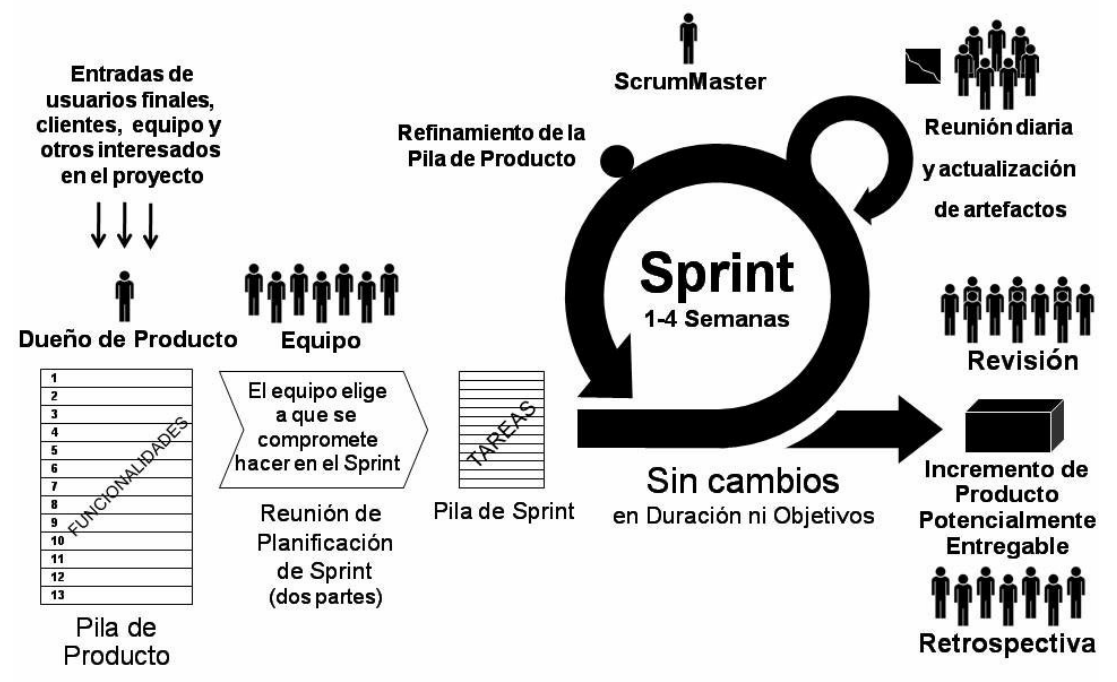
\includegraphics[width=14cm]{./IMAGENES/Scrum} 
		\caption{Cronograma del proyecto}
	\end{center}
\end{figure}


%% ----------------------------------------------------------------------------------------------------------------------------------

%% CRONOGRAMA (PERSONAS, TIEMPO, OTROS RECURSOS) ---------------------------------------------------------------------------------------------------

\section{Cronograma}

\begin{figure}[htb]
	\begin{center}
		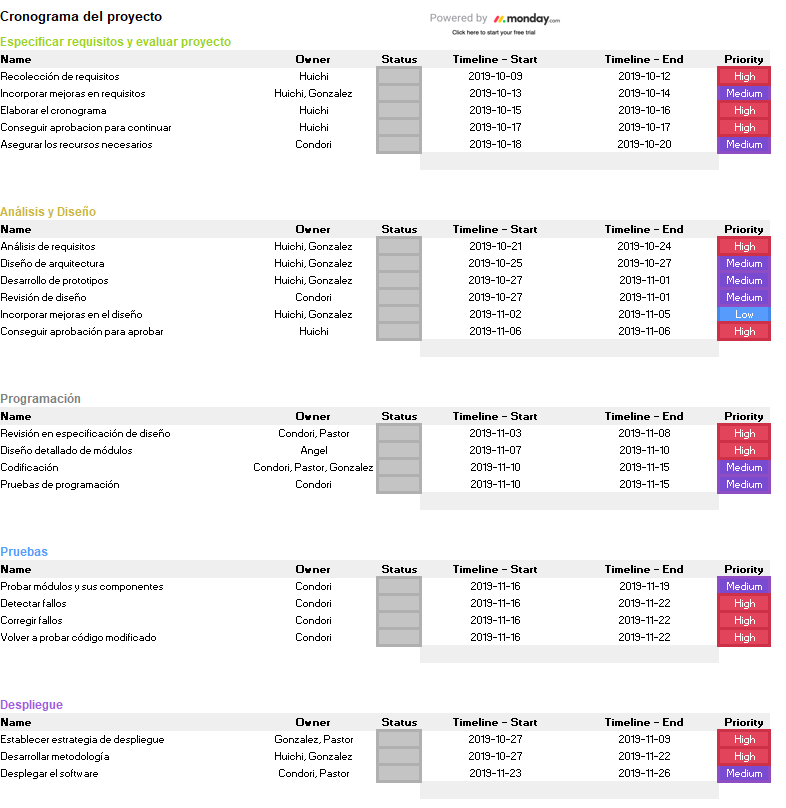
\includegraphics[width=14cm]{./IMAGENES/Gannt} 
		\caption{Cronograma del proyecto}
	\end{center}
\end{figure}

%% ----------------------------------------------------------------------------------------------------------------------------------



%%  REFERENCIAS BIBLIOGRÁFICAS  (OJO NO TOCAR CON CITEP SOLO SE PONEN)------------------------------------------------------------------------------------------
	
	\newpage
	
	\bibliographystyle{apalike} 	%ESTILO
	\bibliography{BIBLIOGRAFIA}	 
	
	
\end{document}
